%  LaTeX support: latex@mdpi.com 
%  For support, please attach all files needed for compiling as well as the log file, and specify your operating system, LaTeX version, and LaTeX editor.

%=================================================================
\documentclass[journal,article,submit,pdftex,moreauthors]{Definitions/mdpi} 

% \usepackage{caption}
\usepackage{graphicx}
\usepackage{amsmath}
\usepackage{algorithmic}
\usepackage[linesnumbered,ruled, vlined]{algorithm2e}
\usepackage{makecell}
\usepackage{threeparttable}
\usepackage{booktabs}
\usepackage{multirow,subfigure}
%--------------------
% Class Options:
%--------------------
%----------
% journal
%----------
% Choose between the following MDPI journals:
% acoustics, actuators, addictions, admsci, adolescents, aerobiology, aerospace, agriculture, agriengineering, agrochemicals, agronomy, ai, air, algorithms, allergies, alloys, analytica, analytics, anatomia, animals, antibiotics, antibodies, antioxidants, applbiosci, appliedchem, appliedmath, applmech, applmicrobiol, applnano, applsci, aquacj, architecture, arm, arthropoda, arts, asc, asi, astronomy, atmosphere, atoms, audiolres, automation, axioms, bacteria, batteries, bdcc, behavsci, beverages, biochem, bioengineering, biologics, biology, biomass, biomechanics, biomed, biomedicines, biomedinformatics, biomimetics, biomolecules, biophysica, biosensors, biotech, birds, bloods, blsf, brainsci, breath, buildings, businesses, cancers, carbon, cardiogenetics, catalysts, cells, ceramics, challenges, chemengineering, chemistry, chemosensors, chemproc, children, chips, cimb, civileng, cleantechnol, climate, clinpract, clockssleep, cmd, coasts, coatings, colloids, colorants, commodities, compounds, computation, computers, condensedmatter, conservation, constrmater, cosmetics, covid, crops, cryptography, crystals, csmf, ctn, curroncol, cyber, dairy, data, ddc, dentistry, dermato, dermatopathology, designs, devices, diabetology, diagnostics, dietetics, digital, disabilities, diseases, diversity, dna, drones, dynamics, earth, ebj, ecologies, econometrics, economies, education, ejihpe, electricity, electrochem, electronicmat, electronics, encyclopedia, endocrines, energies, eng, engproc, entomology, entropy, environments, environsciproc, epidemiologia, epigenomes, est, fermentation, fibers, fintech, fire, fishes, fluids, foods, forecasting, forensicsci, forests, foundations, fractalfract, fuels, future, futureinternet, futurepharmacol, futurephys, futuretransp, galaxies, games, gases, gastroent, gastrointestdisord, gels, genealogy, genes, geographies, geohazards, geomatics, geosciences, geotechnics, geriatrics, grasses, gucdd, hazardousmatters, healthcare, hearts, hemato, hematolrep, heritage, higheredu, highthroughput, histories, horticulturae, hospitals, humanities, humans, hydrobiology, hydrogen, hydrology, hygiene, idr, ijerph, ijfs, ijgi, ijms, ijns, ijpb, ijtm, ijtpp, ime, immuno, informatics, information, infrastructures, inorganics, insects, instruments, inventions, iot, j, jal, jcdd, jcm, jcp, jcs, jcto, jdb, jeta, jfb, jfmk, jimaging, jintelligence, jlpea, jmmp, jmp, jmse, jne, jnt, jof, joitmc, jor, journalmedia, jox, jpm, jrfm, jsan, jtaer, jvd, jzbg, kidneydial, kinasesphosphatases, knowledge, land, languages, laws, life, liquids, literature, livers, logics, logistics, lubricants, lymphatics, machines, macromol, magnetism, magnetochemistry, make, marinedrugs, materials, materproc, mathematics, mca, measurements, medicina, medicines, medsci, membranes, merits, metabolites, metals, meteorology, methane, metrology, micro, microarrays, microbiolres, micromachines, microorganisms, microplastics, minerals, mining, modelling, molbank, molecules, mps, msf, mti, muscles, nanoenergyadv, nanomanufacturing,\gdef\@continuouspages{yes}} nanomaterials, ncrna, ndt, network, neuroglia, neurolint, neurosci, nitrogen, notspecified, %%nri, nursrep, nutraceuticals, nutrients, obesities, oceans, ohbm, onco, %oncopathology, optics, oral, organics, organoids, osteology, oxygen, parasites, parasitologia, particles, pathogens, pathophysiology, pediatrrep, pharmaceuticals, pharmaceutics, pharmacoepidemiology,\gdef\@ISSN{2813-0618}\gdef\@continuous pharmacy, philosophies, photochem, photonics, phycology, physchem, physics, physiologia, plants, plasma, platforms, pollutants, polymers, polysaccharides, poultry, powders, preprints, proceedings, processes, prosthesis, proteomes, psf, psych, psychiatryint, psychoactives, publications, quantumrep, quaternary, qubs, radiation, reactions, receptors, recycling, regeneration, religions, remotesensing, reports, reprodmed, resources, rheumato, risks, robotics, ruminants, safety, sci, scipharm, sclerosis, seeds, sensors, separations, sexes, signals, sinusitis, skins, smartcities, sna, societies, socsci, software, soilsystems, solar, solids, spectroscj, sports, standards, stats, std, stresses, surfaces, surgeries, suschem, sustainability, symmetry, synbio, systems, targets, taxonomy, technologies, telecom, test, textiles, thalassrep, thermo, tomography, tourismhosp, toxics, toxins, transplantology, transportation, traumacare, traumas, tropicalmed, universe, urbansci, uro, vaccines, vehicles, venereology, vetsci, vibration, virtualworlds, viruses, vision, waste, water, wem, wevj, wind, women, world, youth, zoonoticdis 
% For posting an early version of this manuscript as a preprint, you may use "preprints" as the journal. Changing "submit" to "accept" before posting will remove line numbers.

%---------
% article
%---------
% The default type of manuscript is "article", but can be replaced by: 
% abstract, addendum, article, book, bookreview, briefreport, casereport, comment, commentary, communication, conferenceproceedings, correction, conferencereport, entry, expressionofconcern, extendedabstract, datadescriptor, editorial, essay, erratum, hypothesis, interestingimage, obituary, opinion, projectreport, reply, retraction, review, perspective, protocol, shortnote, studyprotocol, systematicreview, supfile, technicalnote, viewpoint, guidelines, registeredreport, tutorial
% supfile = supplementary materials

%----------
% submit
%----------
% The class option "submit" will be changed to "accept" by the Editorial Office when the paper is accepted. This will only make changes to the frontpage (e.g., the logo of the journal will get visible), the headings, and the copyright information. Also, line numbering will be removed. Journal info and pagination for accepted papers will also be assigned by the Editorial Office.

%------------------
% moreauthors
%------------------
% If there is only one author the class option oneauthor should be used. Otherwise use the class option moreauthors.

%---------
% pdftex
%---------
% The option pdftex is for use with pdfLaTeX. Remove "pdftex" for (1) compiling with LaTeX & dvi2pdf (if eps figures are used) or for (2) compiling with XeLaTeX.

%=================================================================
% MDPI internal commands - do not modify
\firstpage{1} 
\makeatletter 
\setcounter{page}{\@firstpage} 
\makeatother
\pubvolume{1}
\issuenum{1}
\articlenumber{0}
\pubyear{2023}
\copyrightyear{2023}
%\externaleditor{Academic Editor: Firstname Lastname}
\datereceived{ } 
\daterevised{ } % Comment out if no revised date
\dateaccepted{ } 
\datepublished{ } 
%\datecorrected{} % For corrected papers: "Corrected: XXX" date in the original paper.
%\dateretracted{} % For corrected papers: "Retracted: XXX" date in the original paper.
\hreflink{https://doi.org/} % If needed use \linebreak
%\doinum{}
%\pdfoutput=1 % Uncommented for upload to arXiv.org

%=================================================================
% Add packages and commands here. The following packages are loaded in our class file: fontenc, inputenc, calc, indentfirst, fancyhdr, graphicx, epstopdf, lastpage, ifthen, float, amsmath, amssymb, lineno, setspace, enumitem, mathpazo, booktabs, titlesec, etoolbox, tabto, xcolor, colortbl, soul, multirow, microtype, tikz, totcount, changepage, attrib, upgreek, array, tabularx, pbox, ragged2e, tocloft, marginnote, marginfix, enotez, amsthm, natbib, hyperref, cleveref, scrextend, url, geometry, newfloat, caption, draftwatermark, seqsplit
% cleveref: load \crefname definitions after \begin{document}

%=================================================================
% Please use the following mathematics environments: Theorem, Lemma, Corollary, Proposition, Characterization, Property, Problem, Example, ExamplesandDefinitions, Hypothesis, Remark, Definition, Notation, Assumption
%% For proofs, please use the proof environment (the amsthm package is loaded by the MDPI class).

%=================================================================
% Full title of the paper (Capitalized)
\Title{PRP: Hardware-Oriented Pattern Replacement Pruning for Deep Neural Networks}

% MDPI internal command: Title for citation in the left column
\TitleCitation{Title}

% Author Orchid ID: enter ID or remove command
\newcommand{\orcidauthorA}{0000-0000-0000-000X} % Add \orcidA{} behind the author's name
%\newcommand{\orcidauthorB}{0000-0000-0000-000X} % Add \orcidB{} behind the author's name

% Authors, for the paper (add full first names)
\Author{Baoyu Chen $^{1,\ddagger,}$*, Diyu Gui $^{2,\ddagger}$ and Yidu Wu $^{3}}

%\longauthorlist{yes}

% MDPI internal command: Authors, for metadata in PDF
\AuthorNames{Baoyu Chen, Diyu Gui and Yidu Wu}

% MDPI internal command: Authors, for citation in the left column
\AuthorCitation{Chen, B.; Gui, D.; Wu, Y.}
% If this is a Chicago style journal: Lastname, Firstname, Firstname Lastname, and Firstname Lastname.

% Affiliations / Addresses (Add [1] after \address if there is only one affiliation.)
\address{%
$^{1}$ \quad College of Mechanical and Electrical Engineering, Hainan Vocational University of Science and Technology,Haikou 571126, China; cby222@126.com\\
$^{2}$ \quad Yangtze Del Region Transformation Center for Adavanced Technological Achevements; dyangzhou22@126.com\\
$^{3}$ \quad Hong Kong Baptist University; wuyidou@gmail.com}

% Contact information of the corresponding author
\corres{Correspondence: cby222@126.com; Tel.: +86-1834-468-6114 (F.L.)}

% Current address and/or shared authorship
%\firstnote{Current address: Affiliation 3.} 
\secondnote{These authors contributed equally to this work.}
% The commands \thirdnote{} till \eighthnote{} are available for further notes


%\simplesumm{} % Simple summary

%\conference{} % An extended version of a conference paper

% Abstract (Do not insert blank lines, i.e. \\) 
\abstract{For wide applications, previous works have developed many model pruning methods to help the deployment of convolutional neural networks (CNNs) in resource-limited platforms. However, the widely unstructured and pattern pruning schemes need extra hardware support to be utilized, while structured pruning ones suffer from accuracy degradation for modifications in network architectures. Thus, we propose a hardware-oriented pattern replacement pruning (PRP) method to compress CNNs considering both compression ratio, model accuracy, and implementation complexity. Compared with previous pruning methods, we have two main advantages: (1) Hardware-friendly kernel replacement: Instead of pruning kernels directly, the PRP approach replaces part of computations with more compact operators originating from the backbone. It compress the network without squeezing the network architecture or introducing any extra operations, leading to better model accuracy and lower implementation complexity compared to prior pruning methods. (2) AutoML-methods for better compression: The meta-learning based neural architecture search (NAS) is introduced into the PRP approach for searching optimal replacement patterns for each convolutional layer, which is conducted by the develop SearchNet. It could enumerate all pruned candidates and evaluate their performances without retraining the large network. To prove the effectiveness, we perform the PRP approach on widely-used ResNet. With a similar accuracy loss, the PRP approach have better compression compared to prior filter pruning algorithms on both CIFAR-10 and ILSVRC-2012 data-sets. Besides, we evaluate the PRP-ResNet on an accelerator supporting sparse CNNs. The proposed PRP approach can achieve better energy efficiency compared to other pruned ResNets with similar sparsity.}

% Keywords
\keyword{Deep neural networks (DNNs); Model Compression; Meta Learning; Pruning, Accelerator} 

% The fields PACS, MSC, and JEL may be left empty or commented out if not applicable
%\PACS{J0101}
%\MSC{}
%\JEL{}

%%%%%%%%%%%%%%%%%%%%%%%%%%%%%%%%%%%%%%%%%%
% Only for the journal Diversity
%\LSID{\url{http://}}

%%%%%%%%%%%%%%%%%%%%%%%%%%%%%%%%%%%%%%%%%%
% Only for the journal Applied Sciences
%\featuredapplication{Authors are encouraged to provide a concise description of the specific application or a potential application of the work. This section is not mandatory.}
%%%%%%%%%%%%%%%%%%%%%%%%%%%%%%%%%%%%%%%%%%

%%%%%%%%%%%%%%%%%%%%%%%%%%%%%%%%%%%%%%%%%%
% Only for the journal Data
%\dataset{DOI number or link to the deposited data set if the data set is published separately. If the data set shall be published as a supplement to this paper, this field will be filled by the journal editors. In this case, please submit the data set as a supplement.}
%\datasetlicense{License under which the data set is made available (CC0, CC-BY, CC-BY-SA, CC-BY-NC, etc.)}

%%%%%%%%%%%%%%%%%%%%%%%%%%%%%%%%%%%%%%%%%%
% Only for the journal Toxins
%\keycontribution{The breakthroughs or highlights of the manuscript. Authors can write one or two sentences to describe the most important part of the paper.}

%%%%%%%%%%%%%%%%%%%%%%%%%%%%%%%%%%%%%%%%%%
% Only for the journal Encyclopedia
%\encyclopediadef{For entry manuscripts only: please provide a brief overview of the entry title instead of an abstract.}

%%%%%%%%%%%%%%%%%%%%%%%%%%%%%%%%%%%%%%%%%%
% Only for the journal Advances in Respiratory Medicine
%\addhighlights{yes}
%\renewcommand{\addhighlights}{%

%\noindent This is an obligatory section in “Advances in Respiratory Medicine”, whose goal is to increase the discoverability and readability of the article via search engines and other scholars. Highlights should not be a copy of the abstract, but a simple text allowing the reader to quickly and simplified find out what the article is about and what can be cited from it. Each of these parts should be devoted up to 2~bullet points.\vspace{3pt}\\
%\textbf{What are the main findings?}
% \begin{itemize}[labelsep=2.5mm,topsep=-3pt]
% \item First bullet.
% \item Second bullet.
% \end{itemize}\vspace{3pt}
%\textbf{What is the implication of the main finding?}
% \begin{itemize}[labelsep=2.5mm,topsep=-3pt]
% \item First bullet.
% \item Second bullet.
% \end{itemize}
%}

%%%%%%%%%%%%%%%%%%%%%%%%%%%%%%%%%%%%%%%%%%
\begin{document}

%%%%%%%%%%%%%%%%%%%%%%%%%%%%%%%%%%%%%%%%%%
% \setcounter{section}{-1} %% Remove this when starting to work on the template.
% \section{How to Use this Template}

% The template details the sections that can be used in a manuscript. Note that the order and names of article sections may differ from the requirements of the journal (e.g., the positioning of the Materials and Methods section). Please check the instructions on the authors' page of the journal to verify the correct order and names. For any questions, please contact the editorial office of the journal or support@mdpi.com. For LaTeX-related questions please contact latex@mdpi.com.%\endnote{This is an endnote.} % To use endnotes, please un-comment \printendnotes below (before References). Only journal Laws uses \footnote.

% % The order of the section titles is different for some journals. Please refer to the "Instructions for Authors” on the journal homepage.

\section{Introduction}\label{sec: intro}

Convolutional neural networks (CNNs) have been extensively applied in multiple computer vision tasks \cite{yolov3,deeplabv3,mask-rcnn}. To increase the accuracy, model sizes of CNNs also enlarge drastically, leading to growing computation and storage complexities. It is hard to deploy large CNNs in resource-limited platforms. Pruning schemes, including unstructured pruning~\cite{M16,ADMM} and structured pruning, is an effective method for model compression. The structured pruning can further be classified into filter pruning~\cite{SFT} and pattern pruning~\cite{banksparse,ese}.

However, the current pruning schemes have different disadvantages in various application scenarios. Unstructured pruning schemes can drastically reduce parameters of the model, but the irregularity of pruned weights harms the performance of hardware implementations, and makes it hard to transfer the reduction of parameters into the processing speedup of algorithms. Filter pruning schemes is able to reduce the model size in a regular way, but the modification of network architecture may lead to unacceptable accuracy loss. To achieve the balance among hardware implementation complexity, model compression, and model accuracy, pattern pruning schemes are proposed. With a pre-set sparse pattern, the pruning scheme helps the algorithm deployment and maintains the model accuracy. However, previous pattern pruning algorithms are closely connected with hardware implementation, while laborious training procedures are introduced to attain tiny networks with complex sparse patterns.

Hence, we design a pattern replacement pruning (PRP) method, utilizing the available compact operators to replace part of original computations. With the pattern replacement, the new network becomes more compact and all computation patterns are selected from the original model, which can be implemented on hardware without extra operator support. Taking ResNets~\cite{M19} as an example, there are $7\times 7$, $3\times 3$, and $1\times 1$ convolutions. The PRP method replaces $3\times 3$ filters with $1\times 1$ filters, which reduces the model computation complexity without extra support in the hardware implementation.

As indicated in ~\cite{lottery}, the architecture left after pruning is more important than the fine-tuned sparse weights, that is to say a pruned network could achieve the same accuracy without inheriting original weights. Thus, the PRP approach aims to find an efficient pruned network architecture, which can achieve the balance between complexity reduction and model accuracy. We introduce neural architecture search (NAS) technique to achieve this goal. Compared to pruning schemes based on human-designed polocies~\cite{M22}, the AutoML-based PRP method can reduce manual works and achieve better performance. Apart from model accuracy and parameter reduction, hardware implementation metrics, such as latency, are also applied as the feedback to search networks~\cite{M21}. 

Inspired by AutoML-based researches, especially the One-Shot model~\cite{M5,OFA} and the Meta-learning method~\cite{Mself}, we develop a SearchNet to evaluate all potential pruned architectures quickly. With the pattern replacement, the reconstructed compact network is generated from the original network. The proportion and position of replacement filters are searched and evaluated by the proposed SearchNet. Fig.~\ref{fig:PRP} illustrates the process of the proposed PRP approach.

\begin{figure} [t]
	\centering
	% Requires \usepackage{graphicx}
	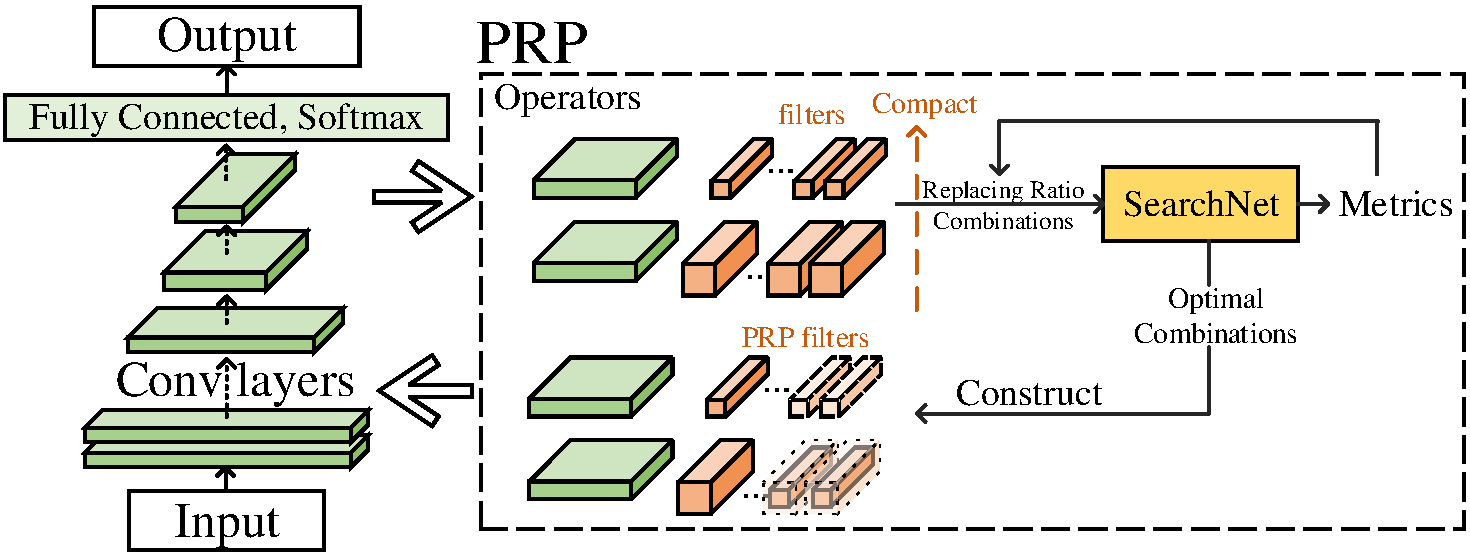
\includegraphics[width=13cm]{figs/overall.pdf}
	\caption{\textbf{Pattern Replacement Pruning Approach.} \textit{Conv layers} is the short for convolutional layers. The green boxes denotes activation of the convolutional layers, and the orange boxes represent filters. We mark the pruned filters as the orange dashed boxes. The proposed SearchNet takes random generated replacing ratio combinations as input, and evaluates the pruned candidates with pre-set metrics. Finally, the optimal combinations can be selected by the SearchNet and utilized to construct the PRP compressed network.}
	\label{fig:PRP}
\end{figure}

To prove the effectiveness, we perform the PRP approach on widely-used ResNet. With a similar accuracy loss, the PRP approach have better compression compared to prior filter pruning algorithms on both CIFAR-10 and ILSVRC-2012 data-sets. Besides, we evaluate the PRP-ResNet on a prior accelerator supporting sparse CNNs. The proposed PRP approach can achieve better energy efficiency compared to other pruned ResNets with similar sparsity.


% We apply our PRP approach on the ResNet~\cite{M19} and evaluate it on both CIFAR-10 and ILSVRC-2012 data-sets. At a similar FLOPs reduction, PRP-pruned ResNet-18 can achieve 2.7\%$\sim$3.5\% higher accuracy than previous pruning methods. For ResNet-50, PRP-pruned network can achieve a 50\% FLOPs reduction without accuracy loss on the CIFAR-10 data-set.

% Moreover, we evaluate the proposed PRP method on an existing CNN accelerator and achieve 14\%$\sim$53\% higher energy efficiency compared to prior pruning works for the hardware-oriented replacement scheme.

% Our contributions lies in three folds:

% 1. We propose a pattern replacement pruning (PRP) approach to compact the network without any additional operations, which can deploy the compressed network to prior accelerators only with little modifications on hardware control.

% 2. To search the optimal compressed network, AutoML methods are introduced into the PRP approach. We develop a SearchNet for the search, evaluation, and generation of the pruned network. Estimated hardware performances are also included in the performance evaluation to convenient the algorithm deployment. Without human design, the PRP approach is able to find the appropriate replacement ratio for every layer.

% 3. To prove the effectiveness, we perform the PRP approach on widely-used ResNet. With a similar accuracy loss, the PRP approach have better compression compared to prior filter pruning algorithms on both CIFAR-10 and ILSVRC-2012 data-sets. Besides, we evaluate the PRP-ResNet on a accelerator supporting sparse CNNs. The proposed PRP approach can achieve better energy efficiency compared to other pruned ResNets with similar sparsity.

% We propose PRP method to allow efficient architecture search for the 1-in-9 pattern pruning, and evaluate the method on a CNN accelerator to prove its validation.

% Compared to filter pruning methods, PRP is more flexible and can achieve a higher accuracy at similar or less FLOPs.

% Compared to pattern pruning methods, PRP introduces AutoML methods, saving human efforts and offering larger search space.


\section{Methodology}\label{sec: method}

\subsection{Pattern Replacement Pruning (PRP)}
Pattern pruning is a suitable alternative for filter pruning due to its flexibility. \cite{banksparse} uses bank-level sparse pattern and~\cite{ese} gives the constrain that paralleled lines should share the same sparsity. Different from filter pruning, pattern pruning will not cause a direct reduction in the model FLOPs unless supported by a specially hardware. 

To collect different information during processing, CNNs usually constructed by filters of multiple kernel sizes. The proposed PRP approach utilizes this property to compress the network architecture by replacing operators with the available compact ones. The replacement can preserve the network architecture compared to the filter pruning approach, minimizing the accuracy loss. Besides, FLOPs reductions of PRP-based networks can be utilized by the existing hardware architecture, for the computation patterns of pruned networks are not extended compared to the original ones.

Take ResNet~\cite{M19} as an example to illustrate the PRP approach. For different applications, ResNets are usually constructed by block structures shown as Fig~\ref{fig:ResNets}, and consists $1\times 1$, $3\times 3$, and $7\times 7$ filters in the network architecture. Utilizing the PRP approach, we mainly replace the $3\times 3$ filters with $1\times 1$ filters in ResNets, which could achieve 50\% FLOPs reduction with negligible accuracy loss. 

\begin{figure} [t]
  \centering
  \subfigure[Basic Block Structures]{
    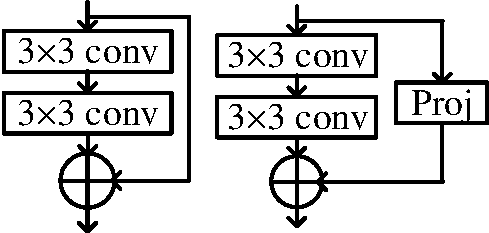
\includegraphics[width=5cm]{figs/resnet-18.pdf}
    \label{fig:basic-block}
  }
  \subfigure[Bottleneck Block Structures]{
    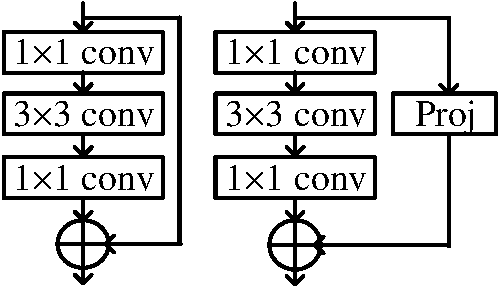
\includegraphics[width=5cm]{figs/resnet-50.pdf}
    \label{fig:bottleneck-block}
  }
  \caption{Block Structures of ResNets. The \textit{Proj} denotes the identity projection utilized in blocks to align the channel numbers of the input and the output.}
  \label{fig:ResNets}
\end{figure} 

For $3\times 3$ filters, the ideal FLOPs reduction of the PRP approach equals to that of the 1-in-9 pattern pruning method, which is achieved by pre-setting 8 zero positions in filters. However, the pruning pattern needs to be selected. For a layer with $N$ $3\times 3$ filters, $M$ filters are pre-set to be pruned. For the PRP method, only the suitable replacement ratio, i.e. $M$, needs to be considered. While for the pattern pruning, $M^9$ different pruning patterns also needs to be selected, which is impossible to find the optimal solution manually. Also, with our experiments, models after the PRP could converge faster and achieve a higher accuracy compared to 1-in-9 pattern pruned ones. 

When processing with compact operators such as $1\times 1$ filters, the PRP approach would replace them with $0\times 0$ filters, i.e. filter pruning. Combining with the filter pruning, the PRP approach can achieve the target FLOPs reduction.

The suitable replacement ratio for each convolutional layer is searched and evaluated by the AutoML methods without human design. Also, the search procedure also prevents the pruning scheme from being trapped in the local optimal. With selected replacement ratio combinations, the PRP compressed network can be reconstructed.

% The accelerator proposed in Section \uppercase\expandafter{\romannumeral5} supports several sparse patterns at inside-kernel level, as shown in Fig.~\ref{fig: PR} (a). We adopt the 1-in-9 sparse pattern on account of compression ratio and hardware consumption. Noticing that channels in one filter share a corporate pruning position considering hardware efficiency.

% \subsection{Pattern Replacement Pruning (PRP)}\label{sec: PRP}
% Assuming a layer with 32 $3\times 3$ filters pruned in a 1-in-9 sparse pattern, it could have $32^9$ pruning modes. It is impossible to find an optimal solution manually. According to our hardware padding mode, $3\times 3$ filters with only one non-zero value is equal to $1\times 1$ filters, as shown in Fig.~\ref{fig: PR} (b). Based on this discover, we propose the Pattern Replacement Pruning (PRP) method. By replacing $3\times 3$ filters with $1\times 1$ filters, the problem is transformed into seeking out a suitable replace ratio for each layer. Models after replacing could converge faster and achieve higher accuracy. AutoML-methods are proved to be efficient for filter pruning, it is also applied for the PRP method, which will be verified in Section \uppercase\expandafter{\romannumeral4}. 

% After we get the replaced model, it should be adjusted to a hardware-supported form. We recover all the replaced $3\times 3$ filters with values offered by these $1\times 1$ filters, leading to a 1-in-9 pattern-pruned model. This method works well on Basic-block-like modules, such as ResNet-18, for $3\times 3$ filters accounting for the majority of the network. But for Bottleneck-like modules, such as ResNet-50, $1\times 1$ filters will harm the general pruning ratio. Thus, we combine filter pruning with the PRP method. Models will be compressed by replacing $3\times 3$ filters and pruning $1\times 1$ filters.

% \begin{figure} [hbt]
% 	\centering
	% Requires \usepackage{graphicx}
% 	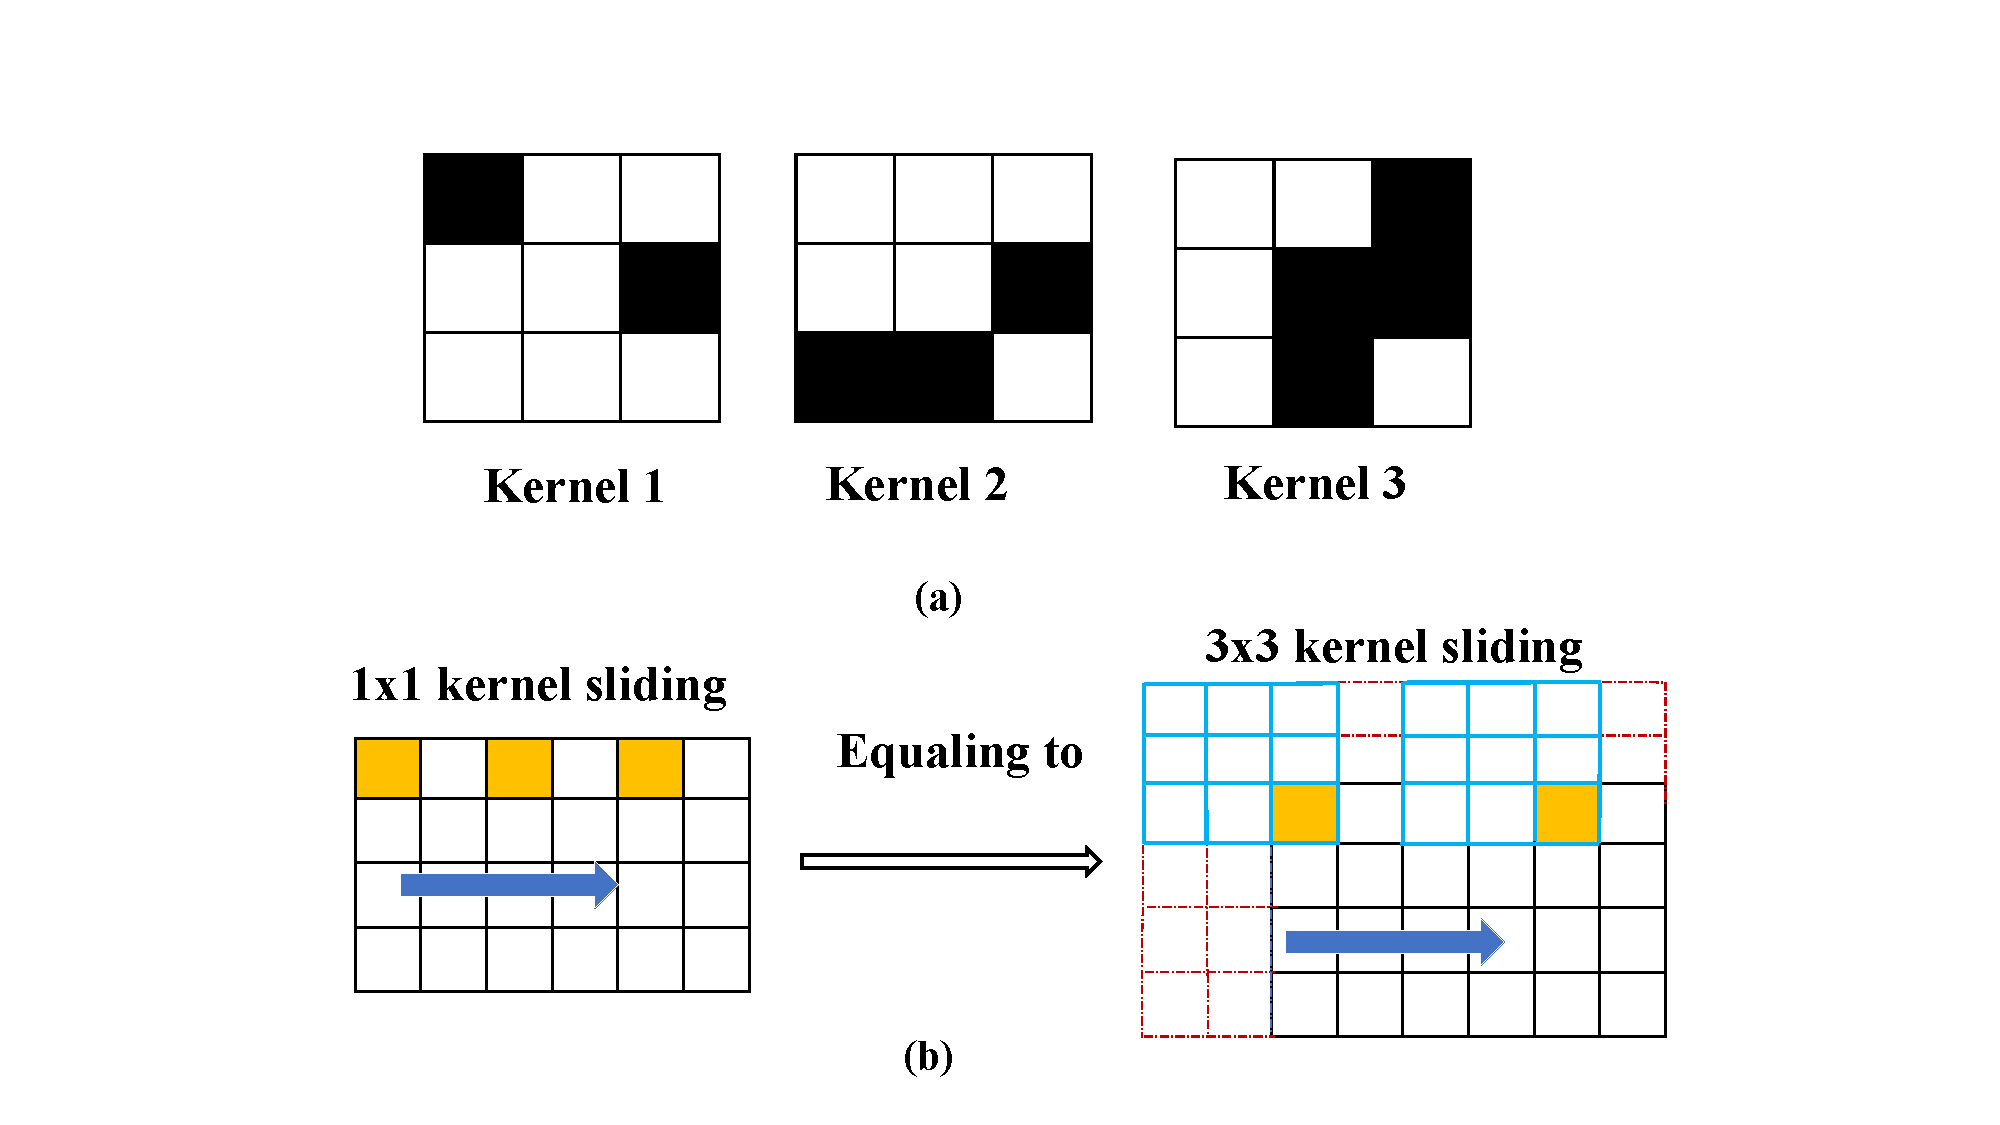
\includegraphics[width=4in]{figs/fig2.pdf}
% 	\caption{\textbf{Illustration of Pattern Pruning.} (a). kernel-level sparse patterns (b). The Computational equivalence of a 1x1 kernel and a pruned 3x3 kernel with the upper left padding \textbf{}.  }\label{fig: PR}
% \end{figure}

\subsection{Training the SearchNet}
Based on the Meta-learning method, we develop a SearchNet to find the suitable replacement ratio by evaluating all the potential pruned architecture quickly. Also, the SearchNet takes compression ratio as input and generates weights for the compressed model. Here, the compression ratio denotes the replacement ratio for $3\times 3$ filters or the filter pruning ratio for $1\times 1$ filters. When searching and evaluating the pruned network, only the SearchNet is evolved, which reduces the retraining efforts of the pruned network. 

Under the conduct of the original network architecture, the SearchNet is built up by replacing convolutional layers by multi-layer perceptron (MLP) architectures. Each MLP architecture contains three fully connected (FC) layers, aiming to generate weights of the corresponding convolutional layer. To ensure the efficiency of the SearchNet, the structure of the MLP architectures are dedicated designed. For block-constructed ResNets, the MLP architectures in the SearchNet are also combined as MLP blocks, which helps to squeeze the search space and increase the training stability. 
 
Take the basic block as an example to illustrate the details of the SearchNet as shown in Fig.\ref{fig: Searchnet}. For a basic block with $64\times 64\times 3\times 3$ filter size, the corresponding MLP architecture is set as three FC layers with sizes of $3\times 16$, $16\times 32$ and $32\times 36864$. Each MLP block receives an input vector composed by compression ratios of adjacent convolutional layers, consisting previous layer and layers of the current block. The included compression ratio of the previous layer is to enlarge the input of the MLP block. With the input replacement ratio vector of (0.1, 0.2, 0.6), the replaced filters are utilized for inference while only weights of the MLP are updated in the backward pass. The update of pruned net can be omitted for all operations are differentiable. The feasibility of this strategy comes from the over-parameter of the MLP structure, allowing the SearchNet to generate corresponding sub-networks according to different compression ratios.
 
\begin{figure} [t]
	\centering
	% Requires \usepackage{graphicx}
	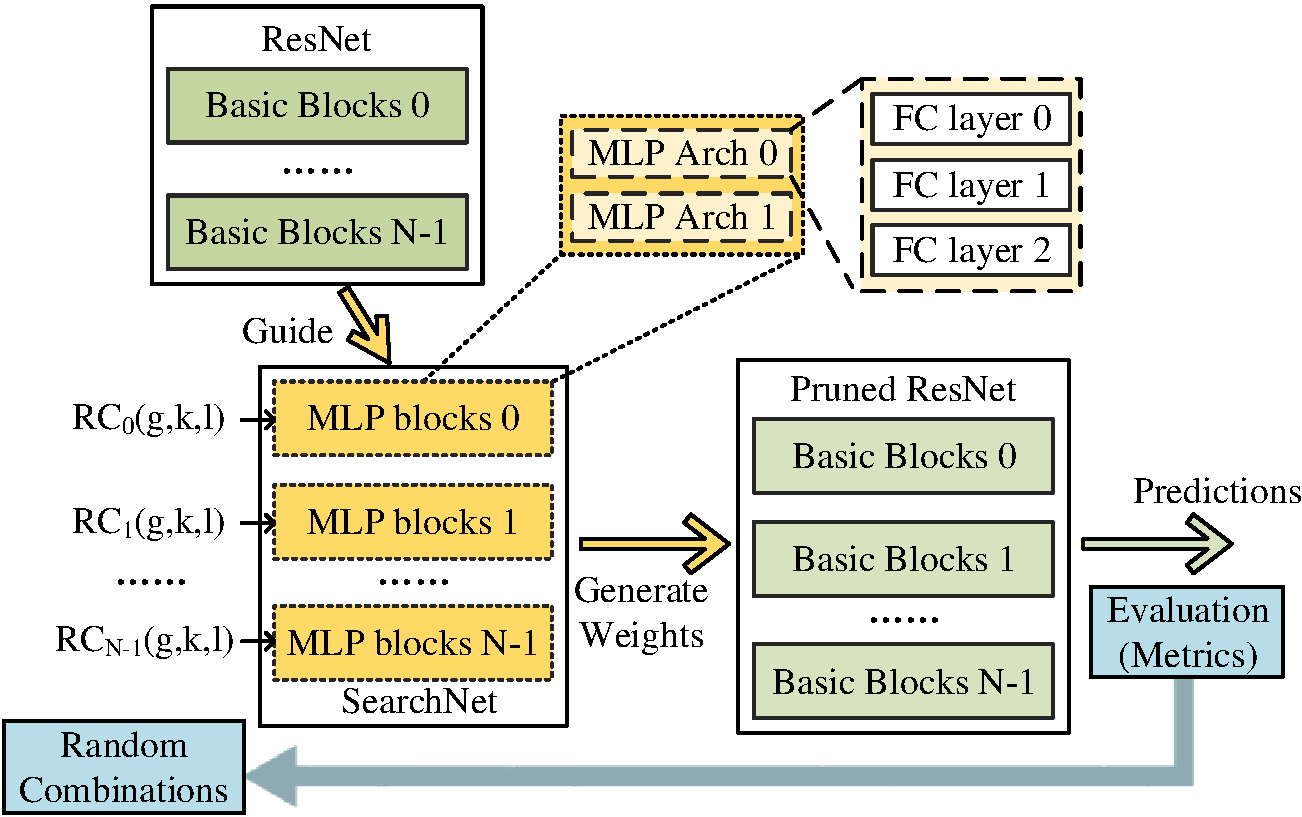
\includegraphics[width=13cm]{figs/SearchNet-arch.pdf}
	\caption{\textbf{Illustration of the SearchNet}, as exampled by a basic block constructed network. \textit{RC} denotes for the replacement ratio for $3\times 3$ filters.}
	\label{fig: Searchnet}
\end{figure}

Furthermore, the proposed PRP method can prune shortcut layers freely compared with previous filter pruning methods. The shortcut layer is utilized in ResNets to address the accuracy degradation problem~\cite{M19}, which is performed by a projection from the block input to its output. For filter pruning methods, extra computations will be introduced in the projection when filter pruning ratios varies in a block. For the proposed PRP approach, when processing with a basic block, we only replace $3\times 3$ filters with $1\times 1$ filters, and output channels remain unchanged compared to the original network. As for a bottleneck block, we keep the $1\times 1$ filters' prune ratio unchanged unless the block contains a downsampling layer. We handle this problem by pruning the downsampling layer and the 3rd layer of the bottleneck block at the same ratio.

\subsection{Architecture Search}
We look for the optimal subnet with the SearchNet. The search and evaluation procedures are processed in an iterative way. In each iteration, $N-10$ random compression ratio combinations for the whole model are generated under the preset pruning ratio, which form the search space. Then, the SearchNet constructs eligible subnets and generates corresponding weights directly, which omits the duplicate retraining of the original network. These generated subnets are evaluated by multiple metrics, such as model accuracy, parameters, and estimated latency of its deployment on hardware. 10 combinations with best performances are selected and combined with the random generated $N-10$ candidates for the next iteration. The whole process ends when the best performance hardly changes, then outputs the optimal subnet.

\section{Experimental Results}\label{sec: experiment}

\subsection{Experiments Settings}
ResNets~\cite{M19} are widely applied nowadays, and most computer visions take residual structures as their backbone. Thus, to prove the effectiveness of our PRP method, we apply it on the widely utilized ResNets and evaluate the PRP-Reset on two benchmarks: CIFAR-10 and ILSVRC-2012. The PRP method could also be extended to other off-the-shelf networks and applied in a variety of deep learning scenarios, which will be explored in the future.


During every mini batch of the training stage, random compression ratio combinations are generated as input vectors of the SearchNet. With forward and backward propagation, the SearchNet could gradually gaining the ability of providing reasonable weights for sub-networks.

\subsection{Results and Comparisons}

To compare the PRP method with normal filter pruning methods, the metrics of model FLOPs and accuracy are utilized as the comparison standards. Compared to network sparsity, the reduction of FLOPs can better reveal the performance of pruning algorithms. As illustrated in the Section, ResNets can be categorized into two types, Type-I: basic-block-based ResNets and Type-II: bottleneck-block-based ResNets. We will demonstrate our works on these two types, separately.

\textbf{Basic-block-based ResNets:} For ResNet-20, 30, and 110 for CIFAR-10 and ResNet-18 for ILSVRC-2012, networks are mainly built by basic blocks with two $3\times 3$ convolutional layers. Besides, several $1\times 1$ filters are also employed in stride=2 blocks for the identical projection from input to output. The PRP method compacts the Type-I ResNets by replacing $3\times 3$ filters with $1\times 1$ ones.

\textbf{Bottleneck-block-based ResNets:} When processing with larger data-sets, instead of basic blocks, ResNets are built by bottleneck blocks to increase network depth with a more compact structure. $1\times 1$ filters account for a large portion in Type-II ResNets. Thus, to reduce more FLOPs of the network, the PRP method compresses $1\times 1$ filters by filter pruning, along with replacing $3\times 3$ filters. That is to say, $1\times 1$ filters are selected and replaced by $0\times 0$ ones in the PRP method for Type-II ResNets. 

%Here we provide a brief description of the dataset we will be using.
Then we provide a brief description of the dataset we will be using:

\textbf{The CIFAR-10 dataset:}
The CIFAR-10 dataset shown in fig~\ref{fig: CIFAR-10} consists of 60000 32x32 colour images in 10 classes, with 6000 images per class. There are 50000 training images and 10000 test images.
The dataset is divided into five training batches and one test batch, each with 10000 images. The test batch contains exactly 1000 randomly-selected images from each class. The training batches contain the remaining images in random order, but some training batches may contain more images from one class than another. Between them, the training batches contain exactly 5000 images from each class.

\begin{figure} [h]
	\centering
	% Requires \usepackage{graphicx}
	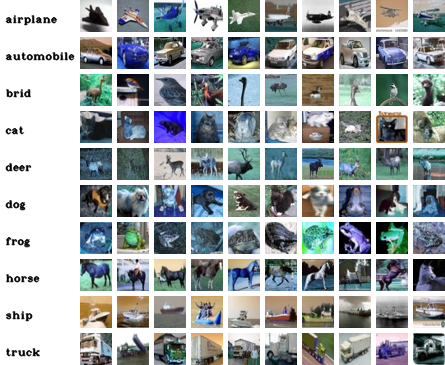
\includegraphics[width=10cm]{figs/CIFAR-10.png}
    \captionsetup{justification=centering}
	\caption{\textbf{Overview of the Dataset CIFAR-10}}
	\label{fig: CIFAR-10}
\end{figure}

\textbf{The ILSVRC2012 dataset:}
ImageNet is a dataset that Feifei Li, a professor at Stanford University, led the construction of in order to solve the problems of overfitting and generalisation in machine learning. Until now, this dataset is still one of the most commonly used datasets for image classification, detection, and localisation in the field of deep learning.
ILSVRC2012 shown in fig~\ref{fig: ILSVRC} refers to a subset of ImageNet-based competitions, i.e., a subset of ImageNet, of which the most commonly used is the 2012 dataset, denoted ILSVRC2012.
The ILSVRC2012 dataset has 1000 classifications with about 1000 images per classification. The total number of these images used for training is about 1.2 million, in addition to a number of images used as a validation set and a test set.ILSVRC2012 contains 50,000 images as a validation set and 100,000 images as a test set.

\begin{figure} [h]
	\centering
	% Requires \usepackage{graphicx}
	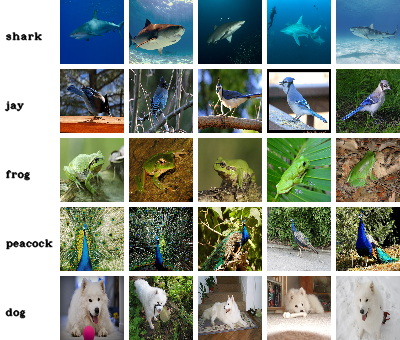
\includegraphics[width=10cm]{figs/ILSVRC.png}
    \captionsetup{justification=centering}
	\caption{\textbf{Overview of the Dataset ILSVRC2012}}
	\label{fig: ILSVRC}
\end{figure}


%over

TABLE~\ref{tab: cifar10} and TABLE~\ref{tab: ilsvrc} present performances of the PRP method deployed on different data-sets. When evaluating on CIFAR-10, the PRP-method can reduce FLOPs to half with merely accuracy loss for ResNet-56, the network can still maintain considerable accuracy when aggressively pruned by about 80{$\%$}. As for ResNet-110, After subtracting 60\% flops, the accuracy loss of the model is only 0.05. In fact, the pruned ResNet-110 has achieved better performance than the original ResNet-56 with similar FLOPs, this also confirms that PRP is an effective pruning scheme, which can obtain small models with higher accuracy and fewer FLOPs from large basic models.



% \usepackage{multirow}
\begin{table}[htb]
\caption{Experiments on CIFAR-10}
\label{tab: cifar10}
\setlength{\tabcolsep}{16pt}
\renewcommand{\arraystretch}{1.3}
\scalebox{1}{
\begin{tabular}{@{}cccccccccc@{}}
\cmidrule(r){1-6}
\multirow{2}{*}{Model} & \multirow{2}{*}{Result} & Base           & Pruned              & Top-1         & FLOPs          &           &           &           &           \\
                       &                         & Top-1          & Top-1               & ↓\%           & ↓\%            &           &           &           &           \\ \cmidrule(r){1-6}
                       & AMC ~\cite{amc}         & 92.8           & 91.9                & 0.9           & 50             &           &           &           &           \\
                       & FPGM ~\cite{fpgm}           & 93.59          & 93.26               & 0.33          & 52.6           &           &           &           &           \\
                       & SFP ~\cite{SFT}           & 93.59          & 93.35               & 0.24          & 52.6           &           &           &           &           \\
RseNet-56              & LFPC ~\cite{lfpc}           & 93.59          & 93.24               & 0.35          & 52.9           &           &           &           &           \\
\textbf{}              & TRP ~\cite{trp}         & 93.14          & 91.62               & 1.52          & 77.82          &           &           &           &           \\
                       & \textbf{Ours}           & \textbf{93.65}          & \textbf{93.61}               & \textbf{0.04}          & \textbf{54.3}            &            &           &          &            \\
                       & \textbf{Ours}           & \textbf{93.65}          & \textbf{92.54}               & \textbf{1.11}         & \textbf{78.6}            &            &           &          &            \\ \cmidrule(r){1-6}
\textbf{}               
                       & Li et al. ~\cite{Li.el}      & 93.53          & 93.30               & 0.23          & 38.60          &           &           &           &           \\
\multirow{2}{*}{RseNet-110}  & SFP ~\cite{SFT}        & 93.50          & 92.74               & 0.76          & 48.5           &           &           &           &           \\
                       & HRank ~\cite{hrank}          & 93.50          & 93.36               & 0.14          & 58.2           &           &           &           &           \\
\textbf{}              & \textbf{Ours}         & \textbf{93.94} & \textbf{93.89} & \textbf{0.05} & \textbf{61.43} & \textbf{} & \textbf{} & \textbf{} & \textbf{} \\ \cmidrule(r){1-6}
\end{tabular}
}
\end{table}

\begin{table}[t]
\caption{Experiments on ILSVRC-2012}
\label{tab: ilsvrc}
\setlength{\tabcolsep}{8pt}
\renewcommand{\arraystretch}{1.3}
\begin{tabular}{@{}ccccccccc@{}}
\toprule
\multirow{2}{*}{Model}     & \multirow{2}{*}{Result}   & Base           & Base                & \multirow{2}{*}{Top-1↓} & \multirow{2}{*}{Top-5↓} & \multirow{2}{*}{FLOPs↓\%} \\
                           &                           & Top-1          & Top-5              &                         &                         &                           \\ \midrule
                           & SFP ~\cite{SFT}              & 76.15          & 92.87                 & 1.54                    & 0.81                    & 41.8                      \\
                           & GAL-0.5 ~\cite{gal}          & 76.15          & 92.87              & 4.20                    & 1.93                    & 43.03                     \\
                           & NISP ~\cite{nisp}             & -              & -                  & 0.89                    & -                       & 44.01                     \\
                           & HP ~\cite{hp}               & 76.01          & 92.93            & 1.14                    & 0.50                    & 50                        \\
                           & MetaPruning ~\cite{metap}      & 76.6           & -                  & 1.2                     & -                       & 51.10                     \\
                           & Autopr ~\cite{autop}          & 76.15          & 92.87            & 1.39                    & 0.72                    & 51.21                     \\
ResNet-50                  & GDP ~\cite{gdp}              & 75.13          & 92.30           & 3.24                    & 1.59                    & 51.30                     \\
                           & FPGM ~\cite{fpgm}             & 76.15          & 92.87            & 1.32                    & 0.55                    & 53.5                      \\
\textbf{}                  & \textbf{Ours}           & \textbf{76.15} & \textbf{92.87}  & \textbf{0.16}           & \textbf{0.08}           & \textbf{54.32}                 \\
                           & C-SGD (extension)~\cite{csgd} & 76.15          & 92.87           & 0.86                    & 0.48                    & 55.44                     \\
                           & C-SGD ~\cite{csgd}           & 75.33          & 92.56            & 0.79                    & 0.47                    & 55.76                     \\
                           & ThiNet ~\cite{thinet}           & 75.30          & 92.20             & 3.27                    & 1.21                    & 55.83                     \\
                           & SASL ~\cite{sasl}             & 76.15          & 92.87            & 1.00                    & 0.40                    & 56.10                     \\
\textbf{}                  & \textbf{Ours}           & \textbf{76.15} & \textbf{92.87} & \textbf{0.43}           & \textbf{0.18}           & \textbf{57.12}            \\
                           & TRP \cite{trp}              & 75.90          & 92.70           & 3.21                    & 1.29                    & 56.52                     \\
                           & LFPC \cite{lfpc}             & 76.15          & 92.87           & 1.69                    & 0.55                    & 60.8                      \\
                           & HRank ~\cite{hrank}            & 76.15          & 92.87            & 4.17                    & 1.86                    & 62.10                     \\
\textbf{}                  & \textbf{Ours}           & \textbf{76.15} & \textbf{92.87}  & \textbf{1.21}           & \textbf{0.43}           & \textbf{61.36}            \\  \bottomrule
\end{tabular}
\end{table}


The results for ILSVRC-2012 also demonstrate the effectiveness of the PRP method. We carefully adjusted the proportion of pruned FLOPs to about 50\%, which is most commonly used in practical applications, and 60\%, which is more aggressive. We can see that PRP maintains good accuracy under the condition of about half FLOPs reduction, which well proves the effectiveness and generalization of PRP on larger data-sets. At the same time, the experimental results also show that adding only very few additional FLOPs pruning on the basis of 50\% will have a harmful impact on model performance. We speculate that this is because the parameters left are not enough to accommodate the knowledge of ILSVRC-2012, which leads to an accelerated decline in model accuracy.

Compared to the other filter pruning schemes, the proposed PRP method can achieve a better balance between the model complexity and accuracy. As shown in TABLE~\ref{tab: cifar10} and TABLE~\ref{tab: ilsvrc}, with a similar FLOPs reduction, the PRP method outperforms prior works in model accuracy. Besides, more FLOPs reduction can be achieved withe a similar accuracy loss. Thus, the PRP method is more flexible and soft, which is very important for model compression.

After our analysis, the PRP method benefits from the \textit{replacement} idea, which compresses the network without squeezing its original network architecture. Also, the compact operators comes from the original network and does not introduce any additional operators, which enables the compressed network be processed by previous accelerators only with a little modification on hardware control.

\subsection{Case Study}
In this section, we conduct ablation studies for further analyzing the proposed pruning method.

\textbf{Direct 1-in-9 pattern pruning} There are two main hinders for implementing the direct 1-in-9 pattern pruning: 1) Select suitable pruning positions for each filter, which includes 9 combinations in a $3\times 3$ kernel; 2) Whether to prune one filter or not. For the first problem, we sum the absolute value of all channels and use the largest one as the maintaining for the filter. For the second obstacle, we set a fixed layer-wise sparse ratio and choose to prune filters with smaller L1-norms. Experiments show that under similar FLOPs, direct pattern pruning tends to suffer a 1\% top-1 accuracy decrease. We summarize two reasons for the accuracy drop: 1) Measuring the importance of a single channel could be quite hard, as it is strongly related to the input feature. Judging by sum of absolute value is not reasonable enough. 2) L1-norm may represent the price of a certain filter, but if most of the greater values occasionally share the same position at kernel-level across differ channels, it could be safely pruned. With PRP, we transform these problems into a combinatorial optimization problem, providing theoretical basis for PRP's validity.

\textbf{Mixed replacement} Inception~\cite{inception} shows that fusing different size of convolution filters could bring performance improvement for CNNs. Consider a layer with 32 $3\times 3$ filters with the replacing ratio $r$ = 0.5. Instead of replacing half of the $3\times 3$ filters with $1\times 1$ filters, we could replace them by a mixed of ten $1\times 1$ filters and six $5\times 5$ depth-wise filters. This solution is feasible at the algorithm level, but due to hardware limitations, we did not experiment with this strategy in this work.


\section{Hardware Implementation}
In this section, we evaluate the proposed PRP method on the existing hardware accelerator to prove its effectiveness. With the same architecture, the proposed PRP approach can achieve the effective speedup compared to the original network and the unstructured pruning approach with a similar sparsity. The acceleration system can also outperforms other structured pruning systems on the overall performance.

\subsection{Hardware Architecture}
The architecture proposed in~\cite{SB} is designed to support the acceleration of unstructured pruned networks. The architecture can be configured by software to support the acceleration of different networks. The overall architecture is shown as Fig.~\ref{fig: ov-arch}.

\begin{figure} [t]
	\centering
	% Requires \usepackage{graphicx}
	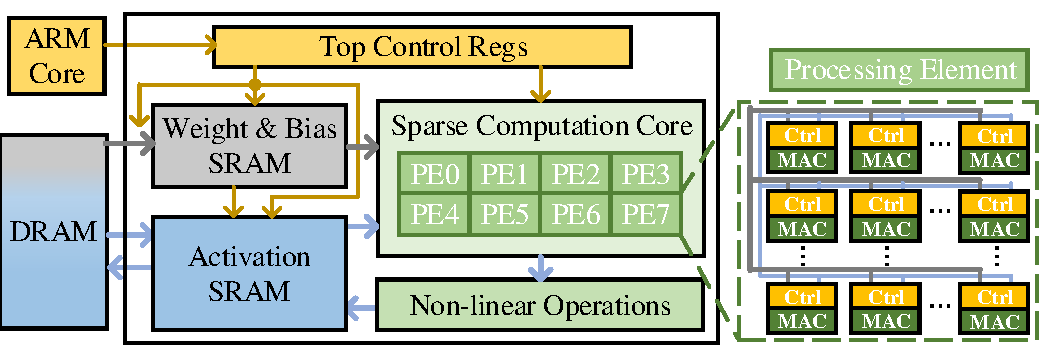
\includegraphics[width=13cm]{figs/arch.pdf}
	\caption{\textbf{The Overall Architecture of the Implemented Accelerator.} The yellow squares and lines denote the hardware control, and will be reconfigured when processing different networks.}
	\label{fig: ov-arch}
\end{figure}

To skip pruned calculations, each PE is driven by the same weight in serial. Paralleled PEs can be configured to process weights from different channels and filters. Due to the irregular distribution of pruned weights in unstructured pruned networks, load imbalance and conflict memory accesses occurs in hardware implementation, leading to the decrease of hardware efficiency. \cite{SB} proposes an off-chip weight pre-processing (WPP) algorithm for pruned weights to improve hardware performance and simplify hardware control. However, extra zeros are introduced in unstructured pruned models after the WPP algorithm, which results in a lower acceleration.

Compressed models after the proposed PRP method have regular distribution of pruned weights, and can be mapped to the architecture without the WPP algorithm. Also, compared to other solution with the co-design of algorithm and hardware, the proposed PRP method is independent from the hardware design and can be implemented on various accelerators only with slightly modification of hardware control.

\subsection{Results and Comparisons}
Evaluated on the the architecture proposed in~\cite{SB}, the PRP method achieves performances shown as Table~\ref{tab:perf} with the same sparsity of 45\% and similar accuracy loss. Compared to work~\cite{shenhaibin}, the proposed method can achieve an improvement of 1.53$\times$ in power efficiency, which gains from the hardware architecture and the specific pattern of the PRP method. Besides, evaluated on the same accelerator, the processing speed of the proposed PRP method is 1.14$\times$ faster than that of the unstructured alternating direction method of multipliers (ADMM)-based~\cite{ADMM} pruning algorithm.
 
\begin{table}[t]
  \centering
  \setlength{\tabcolsep}{8pt}
\renewcommand{\arraystretch}{1.3}
  \begin{threeparttable}
  \caption{The Implementation Performance Comparison of Different Pruning Schemes}
  \label{tab:perf}
    \begin{tabular}{m{2.2cm}<{\centering}||m{2.2cm}<{\centering}|m{2.2cm}<{\centering}|m{2.2cm}<{\centering}|m{2.2cm}<{\centering}}
      \hline\hline
      Works & \cite{shenhaibin} & \cite{SB} & \multicolumn{2}{c}{Ours}\\
      \hline
      Pruning Scheme & ADMM-Structured & ADMM-Unstructured & PRP & None\\
      \hline
      Sparsity & \multicolumn{3}{c}{45\%} & 100\% \\
      \hline
      Quantization & 16-bit & 8-bit & 8-bit & 8-bit \\
      \hline
      Accuracy Loss (top-5) & No Significant Loss & No Loss & No Loss & No Loss \\
      \hline
      Power & 15.4 & 4.6 & 4.6 & 4.6 \\
      \hline
      Images/J & 3.70 & 5.00 & 5.68 & 3.04\\
      \hline
      Computation Efficiency & - & 57.90\% & 65.37\% & 65.07\%\\
      \hline\hline
    \end{tabular}
  \end{threeparttable}
\end{table}

The hardware inefficiency of \cite{SB} is mainly caused by the unsuitable tiling scheme, the under utilization when processing stride=2 convolutions, and communication overhead with external memories. Weights in stride=2 blocks pruned by the PRP approach are more efficient than unstructured pruned ones, leading to the improved hardware efficiency. As shown in TABLE~\ref{tab:perf}, the computation efficiency of the PRP approach is similar to the dense network, which are substantially higher than that of unstructured pruned ones. Implemented with the architecture shown as~\cite{SB}, the hardware efficiency comparisons of different network blocks are shown as Fig. ~\ref{fig: eff}.

\begin{figure} [hbt]
	\centering
	% Requires \usepackage{graphicx}
	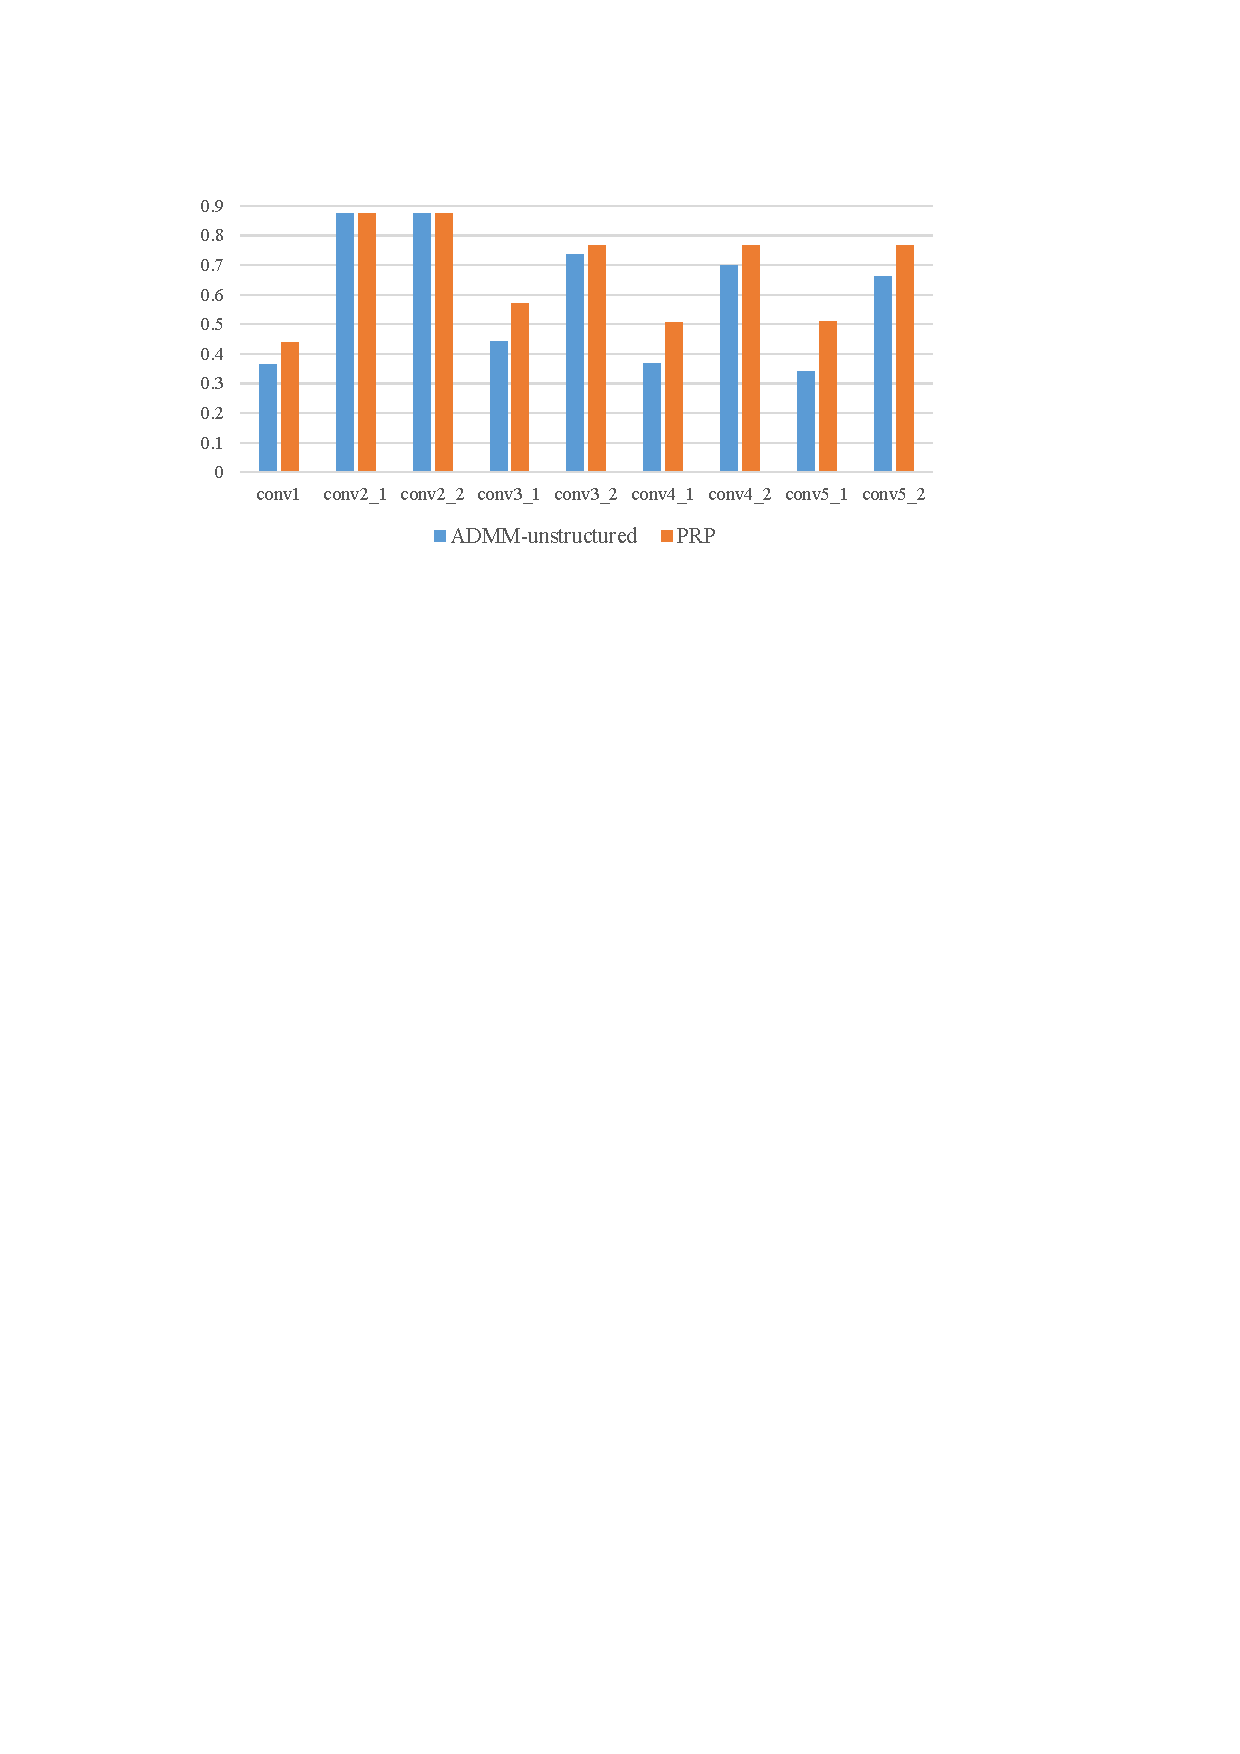
\includegraphics[width=13cm]{figs/computation efficiency.pdf}
	\caption{The Computation Efficiency Comparison of Different Blocks Among Different Pruning Schemes for ResNet-50, where \textit{conv} represents different bottleneck blocks.}
	\label{fig: eff}
\end{figure}

\section{Conclusion}\label{sec: conclusion}
In this paper, we propose a pattern replacement pruning (PRP) approach for hardware-oriented network compression. With the developed pattern replacement idea, the PRP could compact networks without network architecture modification or inducing extra operator, which ensures the model accuracy and helps the hardware deployment of compressed networks. Besides, Auto-ML methods are combined in the PRP approach to save human efforts and achieve better performance. With  experiments on ResNets and comparison with prior works, the PRP approach proves its validation by achieving higher model accuracy at a similar FLOPs reduction. After evaluating on an existing CNN acceleration architecture, the proposed PRP method is able to achieve 14\% higher energy efficiency compared to other pruning schemes.


%%%%%%%%%%%%%%%%%%%%%%%%%%%%%%%%%%%%%%%%%%
\begin{adjustwidth}{-\extralength}{0cm}
%\printendnotes[custom] % Un-comment to print a list of endnotes

\reftitle{References}

\bibliography{ref.bib}
% Please provide either the correct journal abbreviation (e.g. according to the “List of Title Word Abbreviations” http://www.issn.org/services/online-services/access-to-the-ltwa/) or the full name of the journal.
% Citations and References in Supplementary files are permitted provided that they also appear in the reference list here. 

%=====================================
% References, variant A: external bibliography
%=====================================
%\bibliography{your_external_BibTeX_file}

%=====================================
% References, variant B: internal bibliography
%=====================================
% \begin{thebibliography}{999}
% % Reference 1
% % Reference 1
% \bibitem[Xie et al.(2021)]{SB}
% Xie, Xiaoru; Lin, Jun; Wang, Zhongfeng; Wei, Jinghe. An Efficient and Flexible Accelerator Design for Sparse Convolutional Neural Networks. \textit{IEEE Transactions on Circuits and Systems I: Regular Papers}, 2021, 1-14.

% % Reference 4
% \bibitem[Zhu et al.(2020)]{shenhaibin}
% Zhu, Chaoyang; Huang, Kejie; Yang, Shuyuan; Zhu, Ziqi; Zhang, Hejia; Shen, Haibin. An Efficient Hardware Accelerator for Structured Sparse Convolutional Neural Networks on FPGAs. \textit{IEEE Transactions on Very Large Scale Integration (VLSI) Systems}, 2020, \textbf{28}(9), 1953-1965.

% % Reference 5
% \bibitem[Anwar et al.(2017)]{M2}
% Anwar, Sajid; Hwang, Kyuyeon; Sung, Wonyong. Structured Pruning of Deep Convolutional Neural Networks. \textit{ACM Journal on Emerging Technologies in Computing Systems}, 2017, \textbf{13}(3).

% % Reference 6
% \bibitem[Anwar et al.(2016)]{M3}
% Anwar, Sajid; Sung, Wonyong. Compact deep convolutional neural networks with coarse pruning. \textit{arXiv:1610.09639}, 2016.

% % Reference 7
% \bibitem[He et al.(2018)]{M21}
% He, Yihui; Lin, Ji; Liu, Zhijian; Wang, Hanrui; Li, Li-Jia; Han, Song. AMC: AutoML for model compression and acceleration on mobile devices. In \textit{Proceedings of the European Conference on Computer Vision}, 2018, 784-800.

% % Reference 8
% \bibitem[He et al.(2017)]{M22}
% He, Yihui; Zhang, Xiangyu; Sun, Jian. Channel pruning for accelerating very deep neural networks. In \textit{Proceedings of the IEEE International Conference on Computer Vision}, 2017, 1389-1397.


% % Reference 14
% \bibitem[Bender et al.(2018)]{M5}
% Bender, Gabriel; Kindermans, Pieter-Jan; Zoph, Barret; Vasudevan, Vijay; Le, Quoc. Understanding and simplifying one-shot architecture search. In \textit{International Conference on Machine Learning}, 2018, 549-558.

% % Reference 15
% \bibitem[Liu et al.(2019)]{Mself}
% Liu, Zechun; Mu, Haoyuan; Zhang, Xiangyu; Guo, Zichao; Yang, Xin; Cheng, Tim Kwang-Ting; Sun, Jian. MetaPruning: Meta Learning for Automatic Neural Network Channel Pruning. In \textit{Proceedings of the IEEE International Conference on Computer Vision}, 2019.

% % Reference 16
% \bibitem[He et al.(2016)]{M19}
% He, Kaiming; Zhang, Xiangyu; Ren, Shaoqing; Sun, Jian. Deep residual learning for image recognition. In \textit{Proceedings of the IEEE conference on computer vision and pattern recognition}, 2016, 770-778.

% % Reference 18
% \bibitem[Han et al.(2015)]{M16}
% Han, Song; Mao, Huizi; Dally, William J. Deep compression: Compressing deep neural networks with pruning, trained quantization and Huffman coding. \textit{arXiv:1510.00149}, 2015.

% % Reference 20
% \bibitem[He et al.(2018)]{SFT}
% He, Yang; Kang, Guoliang; Dong, Xuanyi; Fu, Yanwei; Yang, Yi. Soft Filter Pruning for Accelerating Deep Convolutional Neural Networks. In \textit{Proceedings of the 27th International Joint Conference on Artificial Intelligence}, 2018, 2234-2240.

% % Reference 21
% \bibitem[Liu et al.(2017)]{NS}
% Liu, Zhuang; Li, Jianguo; Shen, Zhiqiang; Huang, Gao; Yan, Shoumeng; Zhang, Changshui. Learning Efficient Convolutional Networks through Network Slimming. In \textit{IEEE International Conference on Computer Vision}, 2017, 2755-2763.

% % Reference 25
% \bibitem[Cai et al.(2020)]{OFA}
% Cai, Han; Gan, Chuang; Wang, Tianzhe; Zhang, Zhekai; Han, Song. Once-for-All: Train One Network and Specialize it for Efficient Deployment. In \textit{International Conference on Learning Representations}, 2020.

% % Reference 26
% \bibitem[Frankle et al.(2019)]{lottery}
% Frankle, Jonathan; Carbin, Michael. The Lottery Ticket Hypothesis: Finding Sparse, Trainable Neural Networks. In \textit{International Conference on Learning Representations}, 2019.

% % Reference 27
% \bibitem[Wang et al.(2018)]{banksparse}
% Wang, Shuo; Li, Zhe; Ding, Caiwen; Yuan, Bo; Qiu, Qinru; Wang, Yanzhi; Liang, Yun. C-LSTM: Enabling Efficient LSTM Using Structured Compression Techniques on FPGAs. In \textit{Proceedings of the 2018 ACM/SIGDA International Symposium on Field-Programmable Gate Arrays}, 2018, 11–20.

% % Reference 28
% \bibitem[Han et al.(2018)]{ese}
% Han, Song; Kang, Junlong; Mao, Huizi; Hu, Yiming; Li, Xin; Li, Y.; Xie, Dongliang; Luo, Hong; Yao, Song; Wang, Y.; Yang, H.; Dally, W. ESE: Efficient Speech Recognition Engine with Compressed LSTM on FPGA. In \textit{Proceedings of the 2017 ACM/SIGDA International Symposium on Field-Programmable Gate Arrays}, 2018.

% % Reference 29
% \bibitem[Luo et al.(2017)]{thinet}
% Luo, Jian-Hao; Wu, Jianxin; Lin, Weiyao. Thinet: A filter level pruning method for deep neural network compression. In \textit{Proceedings of the IEEE international conference on computer vision}, 2017, 5058-5066.

% % Reference 30
% \bibitem[Dong et al.(2017)]{MiL}
% Dong, Xuanyi; Huang, Junshi; Yang, Yi; Yan, Shuicheng. More is Less: A More Complicated Network with Less Inference Complexity. In \textit{2017 IEEE Conference on Computer Vision and Pattern Recognition}, 2017, 1895-1903.

% % Reference 31
% \bibitem[Szegedy et al.(2016)]{inception}
% Szegedy, Christian; Vanhoucke, Vincent; Ioffe, Sergey; Shlens, Jonathon; Wojna, Zbigniew. Rethinking the Inception Architecture for Computer Vision. In \textit{2016 IEEE Conference on Computer Vision and Pattern Recognition}, 2016.

% % Reference 32
% \bibitem[Zagoruyko and Komodakis(2016)]{Zagoruyko}
% Zagoruyko, Sergey; Komodakis, Nikos. Wide residual networks. In \textit{The British Machine Vision Conference}, 2016.

% % Reference 33
% \bibitem[He et al.(2016)]{kaiming}
% He, Kaiming; Zhang, Xiangyu; Ren, Shaoqing; Sun, Jian. Identity mappings in deep residual networks. In \textit{Proceedings of the European Conference on Computer Vision}, 2016.


% % Reference 36
% \bibitem[Redmon and Farhadi(2018)]{yolov3}
% Redmon, Joseph; Farhadi, Ali. YOLOv3: An Incremental Improvement. \textit{arXiv:1804.02767}, 2018.

% % Reference 37
% \bibitem[Chen et al.(2018)]{deeplabv3}
% Chen, Liang-Chieh; Zhu, Yukun; Papandreou, George; Schroff, Florian; Adam, Hartwig. Encoder-Decoder with Atrous Separable Convolution for Semantic Image Segmentation. In \textit{Proceedings of the European Conference on Computer Vision}, 2018.

% % Reference 38
% \bibitem[He et al.(2017)]{mask-rcnn}
% He, Kaiming; Gkioxari, Georgia; Dollár, Piotr; Girshick, Ross. Mask R-CNN. In \textit{2017 IEEE International Conference on Computer Vision}, 2017, 2980-2988.

% % Reference 39
% \bibitem[Zhang et al.(2018)]{ADMM}
% Zhang, Tianyun; Ye, Shaokai; Zhang, Kaiqi; Tang, Jian; Wen, Wujie; Fardad, Makan; Wang, Yanzhi. A Systematic DNN Weight Pruning Framework Using Alternating Direction Method of Multipliers. \textit{Lecture Notes in Computer Science}, 2018, 191–207.

% % Reference 40
% \bibitem[Zhang et al.(2016)]{cambricon}
% Zhang, Shijin; Du, Zidong; Zhang, Lei; Lan, Huiying; Liu, Shaoli; Li, Ling; Guo, Qi; Chen, Tianshi; Chen, Yunji. Cambricon-X: An accelerator for sparse neural networks. In \textit{2016 49th Annual IEEE/ACM International Symposium on Microarchitecture (MICRO)}, 2016, 1-12.



% \end{thebibliography}

% If authors have biography, please use the format below
%\section*{Short Biography of Authors}
%\bio
%{\raisebox{-0.35cm}{\includegraphics[width=3.5cm,height=5.3cm,clip,keepaspectratio]{Definitions/author1.pdf}}}
%{\textbf{Firstname Lastname} Biography of first author}
%
%\bio
%{\raisebox{-0.35cm}{\includegraphics[width=3.5cm,height=5.3cm,clip,keepaspectratio]{Definitions/author2.jpg}}}
%{\textbf{Firstname Lastname} Biography of second author}

% For the MDPI journals use author-date citation, please follow the formatting guidelines on http://www.mdpi.com/authors/references
% To cite two works by the same author: \citeauthor{ref-journal-1a} (\citeyear{ref-journal-1a}, \citeyear{ref-journal-1b}). This produces: Whittaker (1967, 1975)
% To cite two works by the same author with specific pages: \citeauthor{ref-journal-3a} (\citeyear{ref-journal-3a}, p. 328; \citeyear{ref-journal-3b}, p.475). This produces: Wong (1999, p. 328; 2000, p. 475)

%%%%%%%%%%%%%%%%%%%%%%%%%%%%%%%%%%%%%%%%%%
%% for journal Sci
%\reviewreports{\\
%Reviewer 1 comments and authors’ response\\
%Reviewer 2 comments and authors’ response\\
%Reviewer 3 comments and authors’ response
%}
%%%%%%%%%%%%%%%%%%%%%%%%%%%%%%%%%%%%%%%%%%
\PublishersNote{}
\end{adjustwidth}
\end{document}

